\chapter{Results}\label{chp:results}

In this chapter, we present the results of different networks. Every section from \ref{sec:res} to \ref{sec:gogl} presents the results for each network. every section is divided in three subsection: one in which we discuss the results of different initialization one where we discuss the results of different optimizers and one in which the results for different classes are presented. 
\section{Resnet}\label{sec:res}
\subsection{Initialization}
For every class, we tested our network with either random initialization or with using pretrained weights. In Table \ref{tab:resinit}, we can see the best accuracy on validation and test set, the number of epochs for training for each class. Then on Figure\ref{fig:}, we plotted the accuracy, F1 score, and average training and validation loss for each class.  

\begin{table}
\caption{\label{tab:vitus-realm-user} The results of training ResNet18 using random initialization or pretrained weights with Adamax as optimizer}
\centering
\begin{tabular}[b]{| l | l | l | l | l |}
\hline
    Initialization & Class & Validation accuracy & Test accuracy & Epochs\ \\ \hline
    \multirow{}{}{Pretrained Weights} & Dunham &  62\% & 34\% & 50 \\ 
    & Porosity & 75\% & 45\% &  50 \\
    &DRT & 75\% & 45\% &  50 \\
    &Components & 75\% & 45\% &  50 \\ \hline
     \multirow{}{}{Random} & Dunham &  62\% & 34\% & 50 \\
    & Porosity & 75\% & 45\% &  50 \\
    &DRT & 75\% & 45\% &  50 \\
    &Components & 75\% & 45\% &  50 \\ \hline
    
\end{tabular} 
\end{table}

\begin{figure}
    \centering
    \begin{minipage}{0.4\textwidth}
        \centering
        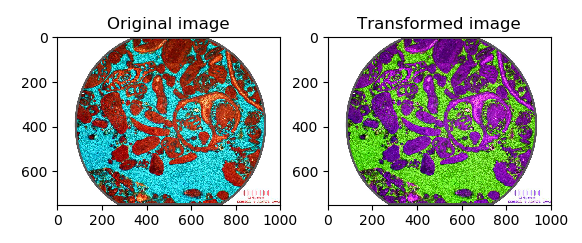
\includegraphics[width=0.9\textwidth]{figures/03-hue05.PNG} % first figure itself
        \caption{Resnet18 trained on porosity class. The lines in green and red are for pretrained weights and yellow  and blue for random initialization. The top plot is the accuracy and the bottom plot is training  and loss accuracy. }\label{fig:classes}
    \end{minipage}
    \begin{minipage}{0.4\textwidth}
        \centering
        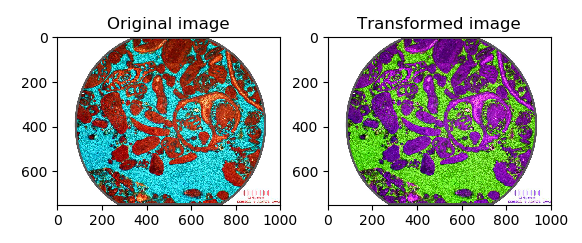
\includegraphics[width=0.9\textwidth]{figures/03-hue05.PNG} % second figure itself
        \caption{Image after ColorJitter with contrast to 1, all others parameters to 0}\label{fig:litandstruc}
    \end{minipage}
    \begin{minipage}{0.4\textwidth}
        \centering
        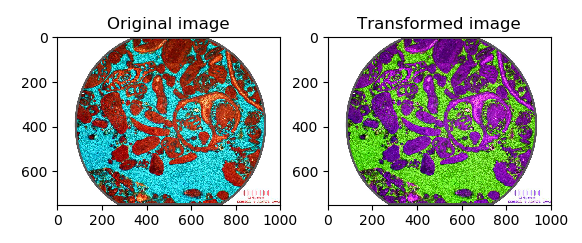
\includegraphics[width=0.9\textwidth]{figures/03-hue05.PNG} % second figure itself
        \caption{Image after ColorJitter with saturation to 0.6, all others parameters to 0}\label{fig:litandstruc}
    \end{minipage}
    \begin{minipage}{0.4\textwidth}
        \centering
        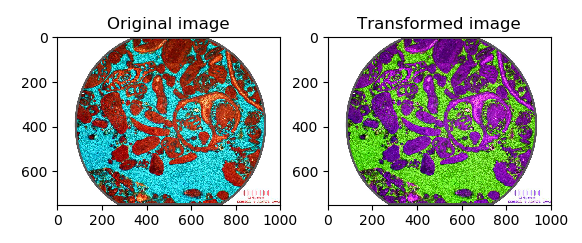
\includegraphics[width=0.9\textwidth]{figures/03-hue05.PNG} % second figure itself
        \caption{Image after ColorJitter with hue to 0.5, all others parameters to 0}\label{fig:litandstruc}
    \end{minipage}
\end{figure}

\subsection{Optimizer}
\subsection{Classification}
\section{AlexNet}\label{sec:aleX}
\subsection{Initialization}
\subsection{Optimizer}
\subsection{Classification}
\section{GoogleNet}\label{sec:gogl}
\subsection{Initialization}
\subsection{Optimizer}
\subsection{Classification}